In this section, we show how our model can describe the most widely used substream management framework called {\em pucntuations}. We also prove specific properties that are inherent to any implementation of the punctuation framework. 

\subsection{Framework Overview}

The main idea behind the punctuation framework is to inject special data elements $\mathcal{P}^{pred}$ into the data stream one per substream. These elements, called punctuations, flow down the workflow as ordinary data elements. The injector promises that all elements after punctuations will not satisfy the predicate. Hence, the punctuation itself defines the ``border'' of a substream.

Figure~\ref{punctuations_scheme} illustrates the punctuation framework. Punctuations are delimiters between the substream elements and all other items. Green elements indicate elements that belong to some substream, while red elements do not.

\begin{figure}[t]
  \centering
  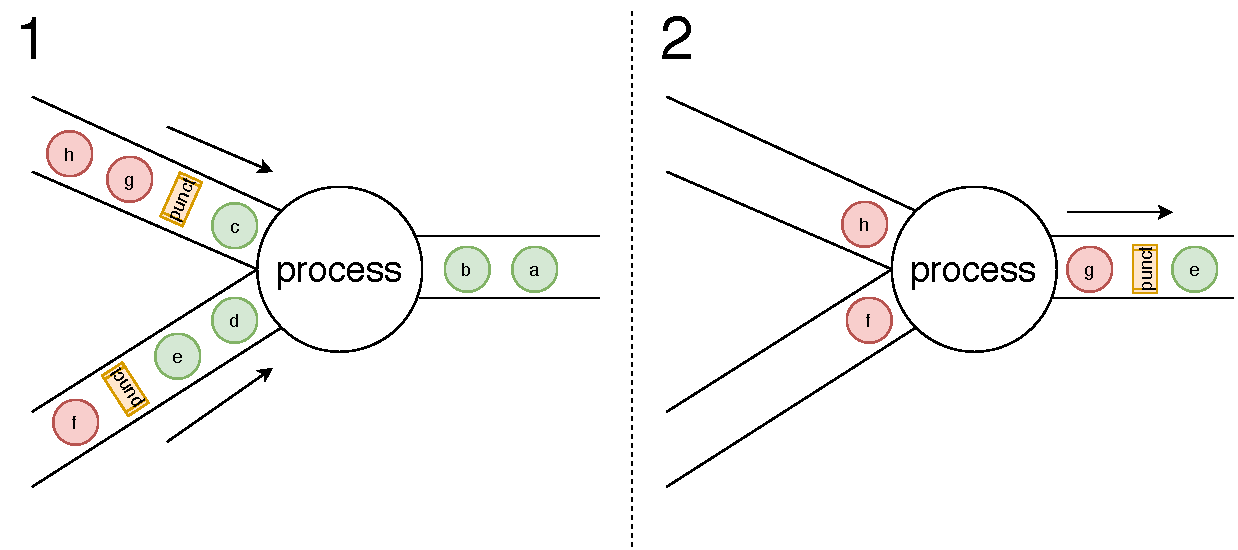
\includegraphics[width=0.80\textwidth]{Chapters/SubstreamConsistency/pics/punctuations-scheme.pdf}
  \caption{Punctuations handling by a single process}
  \label{punctuations_scheme}
\end{figure}

Processes within SPE do not apply user-defined operators to punctuations. Instead, each process $p$ propagates punctuation messages $\mathcal{P}_{pq}^{pred}$ to all outgoing channels $c_{pq} \in O_p$  when it receives corresponding punctuations from all input channels $I_p$.

\subsection{Substream Termination Events}

\begin{lemma}
Generating an event by the following rule ensures the soft bound of a substream $pred$:
\begin{equation}
\forall q \in I_p, \exists \mathcal{P}^{pred}_{qp} \in B_p, \forall M\in B_p : \neg pred(M) \vee dst(M) \ne p
\end{equation}
\end{lemma}

\begin{proof}
We can use indirect proof. Let $\langle proc, p, M^*, M' \rangle$ be a processing event that happens after the soft bound termination event but $pred(M^*)$. In other words, a message $M^*, pred(M^*)$ arrived after all punctuations for the predicate $pred$ had arrived. According to the definition of a distributed system from Section~\ref{fs-acker-spe-model}, message $M^*$ could emerge either from the mailbox of a process or incoming channels. The emergence from the mailbox contradicts the condition of the termination event generation rule $\forall M\in B : \neg pred(M) \vee dst(M) \ne p$.
Conversely, if an element comes from an incoming channel, we can track its path through the system from a data source to the channel (processing path). Because of broadcasts on each step, punctuations travel all possible paths in the system, including the path that traveled the element. Along this path, they were reordered. It could happen either during transmission or during processing. The first hypothesis contradicts the FIFO nature of communication channels. The second one is impossible due to the definition of the processing model that protects a processing order. We have excluded all possible ways of getting event $M^*$ and must reject the initial hypothesis.
\end{proof}

To satisfy the firm bound guarantee, the mailbox controller should block the processing of all incoming messages from a channel as soon as it receives punctuation from this channel. In~\cite{Carbone:2017:SMA:3137765.3137777}, such behavior is called {\em watermark (punctuation) alignment}. Formally we can rewrite this requirement in terms of event ordering:

\begin{lemma}
A soft bound becomes firm if a process event order satisfies the following conditions:
\begin{equation}
\label{eq:firm_condition}
\forall e_1, e_2 = \langle recv, p, \mathcal{P}^{pred}_{q_{1,2}p} \rangle, \nexists e' = \langle proc, p, M_{q_1p}, M' \rangle, e_1 <_p e' <_p e_2
\end{equation}
\end{lemma}
\begin{proof}
Suppose a message $M_{qp}$ of the next substream was processed after the last element of the current substream but before the generation of a bound event. This message either came from the channel $q$ before the punctuation from that channel or was processed before all channels delivered their punctuations. The first case could happen if $M_{qp}$ was reordered with the punctuation along the processing path and contradicts FIFO processing logic (see previous proof for details). The second case is impossible because of processing limitations introduced by~\ref{eq:firm_condition}.
\end{proof}

\subsection{Properties of the Punctuation Framework}

The design of the punctuation framework implies two important properties:

\begin{enumerate}
    \item {\bf Lack of cyclic dataflows support.} Although there are techniques that extend punctuations for state snapshotting of iterative processing~\cite{Carbone:2017:SMA:3137765.3137777}, the termination of a general substream cannot be determined using the punctuation framework if an execution graph contains cycles.
    \item {\bf Network traffic complexity quadratically depends on the number of processes.} As we demonstrated above, each process waits for punctuations from all incoming network channels delivers. It leads to high network traffic overhead if all processes are interconnected.
\end{enumerate}

\begin{lemma}
The punctuation framework cannot determine a substream termination of an execution graph if the graph contains a cycle.
\end{lemma}
\begin{proof}
If we have a cycle in the processing graph, we can find a process that receives input from the latter steps of the cycle (back-link). This process will propagate a punctuation element when all incoming channels have received their punctuation elements. Due to the cycle, this punctuation element processing path contains the process itself (as a starting element of the cycle). It means that we need the punctuation to be already generated to generate it. We obtained a contradiction.
\end{proof}

Despite the previous Lemma, some punctuation-based systems report support of cyclic workflows. One can practically achieve it by limiting the number of possible entrances into the cycle by some $m$. With this limitation, we can roll out the cycle with repeating fragments of the cycle $m$ times. The first block is then connected to the input of the cycle, and the last element of the cycle to two elements: repetition entrance and the output of the cycle. Repetitions are organized the same way. Theoretically, this cycle representation is a DAG so that the punctuation mechanism can serve it.

For example, the technique proposed in~\cite{Carbone:2017:SMA:3137765.3137777} allows SPEs to use punctuations for the state snapshotting problem. The main idea of this technique is to include in a snapshot all in-transit elements (possibly from previous epochs) within a cycle and then resend them on rollback. It is the specific form of the limitation on the number of possible entrances with $m=1$.

\begin{lemma}
Network traffic complexity for this method is $O(K|\Pi|^2)$, where $|\Pi|$ is the number of processes and $K$ is the number of substreams if an SPE distributes the work among processes evenly.
\end{lemma}
\begin{proof}

Even the soft bound event requires receiving punctuations from all incoming network channels. If a distributed stream processing engine balances the work evenly among the processes, all processes are interconnected. Therefore, each active process should broadcast punctuations to all other processes. Assuming that all processes handle the elements belonging to the predicate, the transmission complexity of punctuation elements is $O(K|\Pi|^2)$. Therefore, if the number of existing substreams is $K$, then the network traffic complexity for the punctuation framework is $O(K|\Pi|^2)$ because each process should broadcast punctuations for each substream. 

\end{proof}

Several promising directions exist for improving the network traffic complexity for the punctuation framework. Firstly, one can batch punctuations for several substreams if they do not require independent termination events. It can reduce network complexity to $O(\frac{K}{B}|\Pi|^2)$ where B is a batching frequency. On the other hand, this approach is unsuitable for all substream types (e.g., it cannot be applied for epochs) and can increase the latency between the substream end and the termination event while keeping the quadratic dependency on the number of nodes.

Secondly, it is possible to attach punctuations to all regular input data elements. In this case, there can be no extra traffic in terms of messages at all. However, it makes the latency between the substream end and the termination event unpredictable because some network channels can rarely be used.

Both mentioned optimization ideas have significant trade-offs and require deep theoretical and experimental research. We do not elaborate on optimization ideas in this work, leaving them for future work.
